\section{Networks-On-Chip}\label{sec:networkonchipfun}
\textit{Networks-on-Chip} (or \textit{\glspl{noc}} for short) are a method of interconnecting components on a chip. Typically employed on
\textit{Multi-Processor Systems-on-Chip (\glspl{mpsoc})} \cites(e.g.)(){ivanov05nocintroduction}{biswas15routerattack}{tatas16designingnocs}, they
provide the communication infrastructure for \textit{processing elements (\glspl{pe})} and possibly other \gls{ip} cores.

The topology of a \gls{noc} can vary. Researchers usually work with a 2D mesh topology
\cites(e.g.)(){frey17hardenednoc}{kumar02networkonchip}{fernandes16nocrouting}{boraten16packetsecurity}, which will also be used throughout this thesis.
In this case, each network node is connected to its four neighbors (excluding the boundary nodes).

A node typically consists of a processing element (often referred to as an \textit{\gls{ip} core} or just \textit{core}), a network interface
(\textit{\gls{ni}}), and a router. \cite{dally01routepacketsnotwires} The router manages the connections to neighboring nodes while also allowing
the local processing element to communicate with the network through the network interface. An example of this architecture is given in Figure
\vref{fig:nocexample}.

Compared to traditional bus-based interconnect systems, \glspl{noc} can provide a lot of advantages, especially for many-core systems.
\cite[5\psqq]{tatas16designingnocs} One big advantage is scalability; because the cores do not share a global bus, \enquote{local performance is not
degraded} \cite[6]{tatas16designingnocs} as more components are added, and \enquote{aggregated bandwidth scales with the network size}
\cite[6]{tatas16designingnocs}.

In addition, the absence of global interconnection wires facilitates the use of different clock domains. This enables the implementation of the
\textit{globally asynchronous, locally synchronous (\gls{gals})} paradigm, which becomes increasingly important in chip design.
\cites[3]{kumar02networkonchip}[2]{ivanov05nocintroduction}

Furthermore, with the constantly increasing design complexity of modern chips \cite{mack11mooreslaw}, specialized on-chip
interconnections become infeasible to implement. Designing such a system \enquote{would take too much time and mapping of applications to dedicated
architectures would be impossible} \cite[1]{kumar02networkonchip}. In contrast, \glspl{noc} aims to be general purpose interconnect systems; they
\enquote{facilitate […] modularity by defining a standard interface} \cite[1]{dally01routepacketsnotwires}.

\begin{figure}
    \centering
    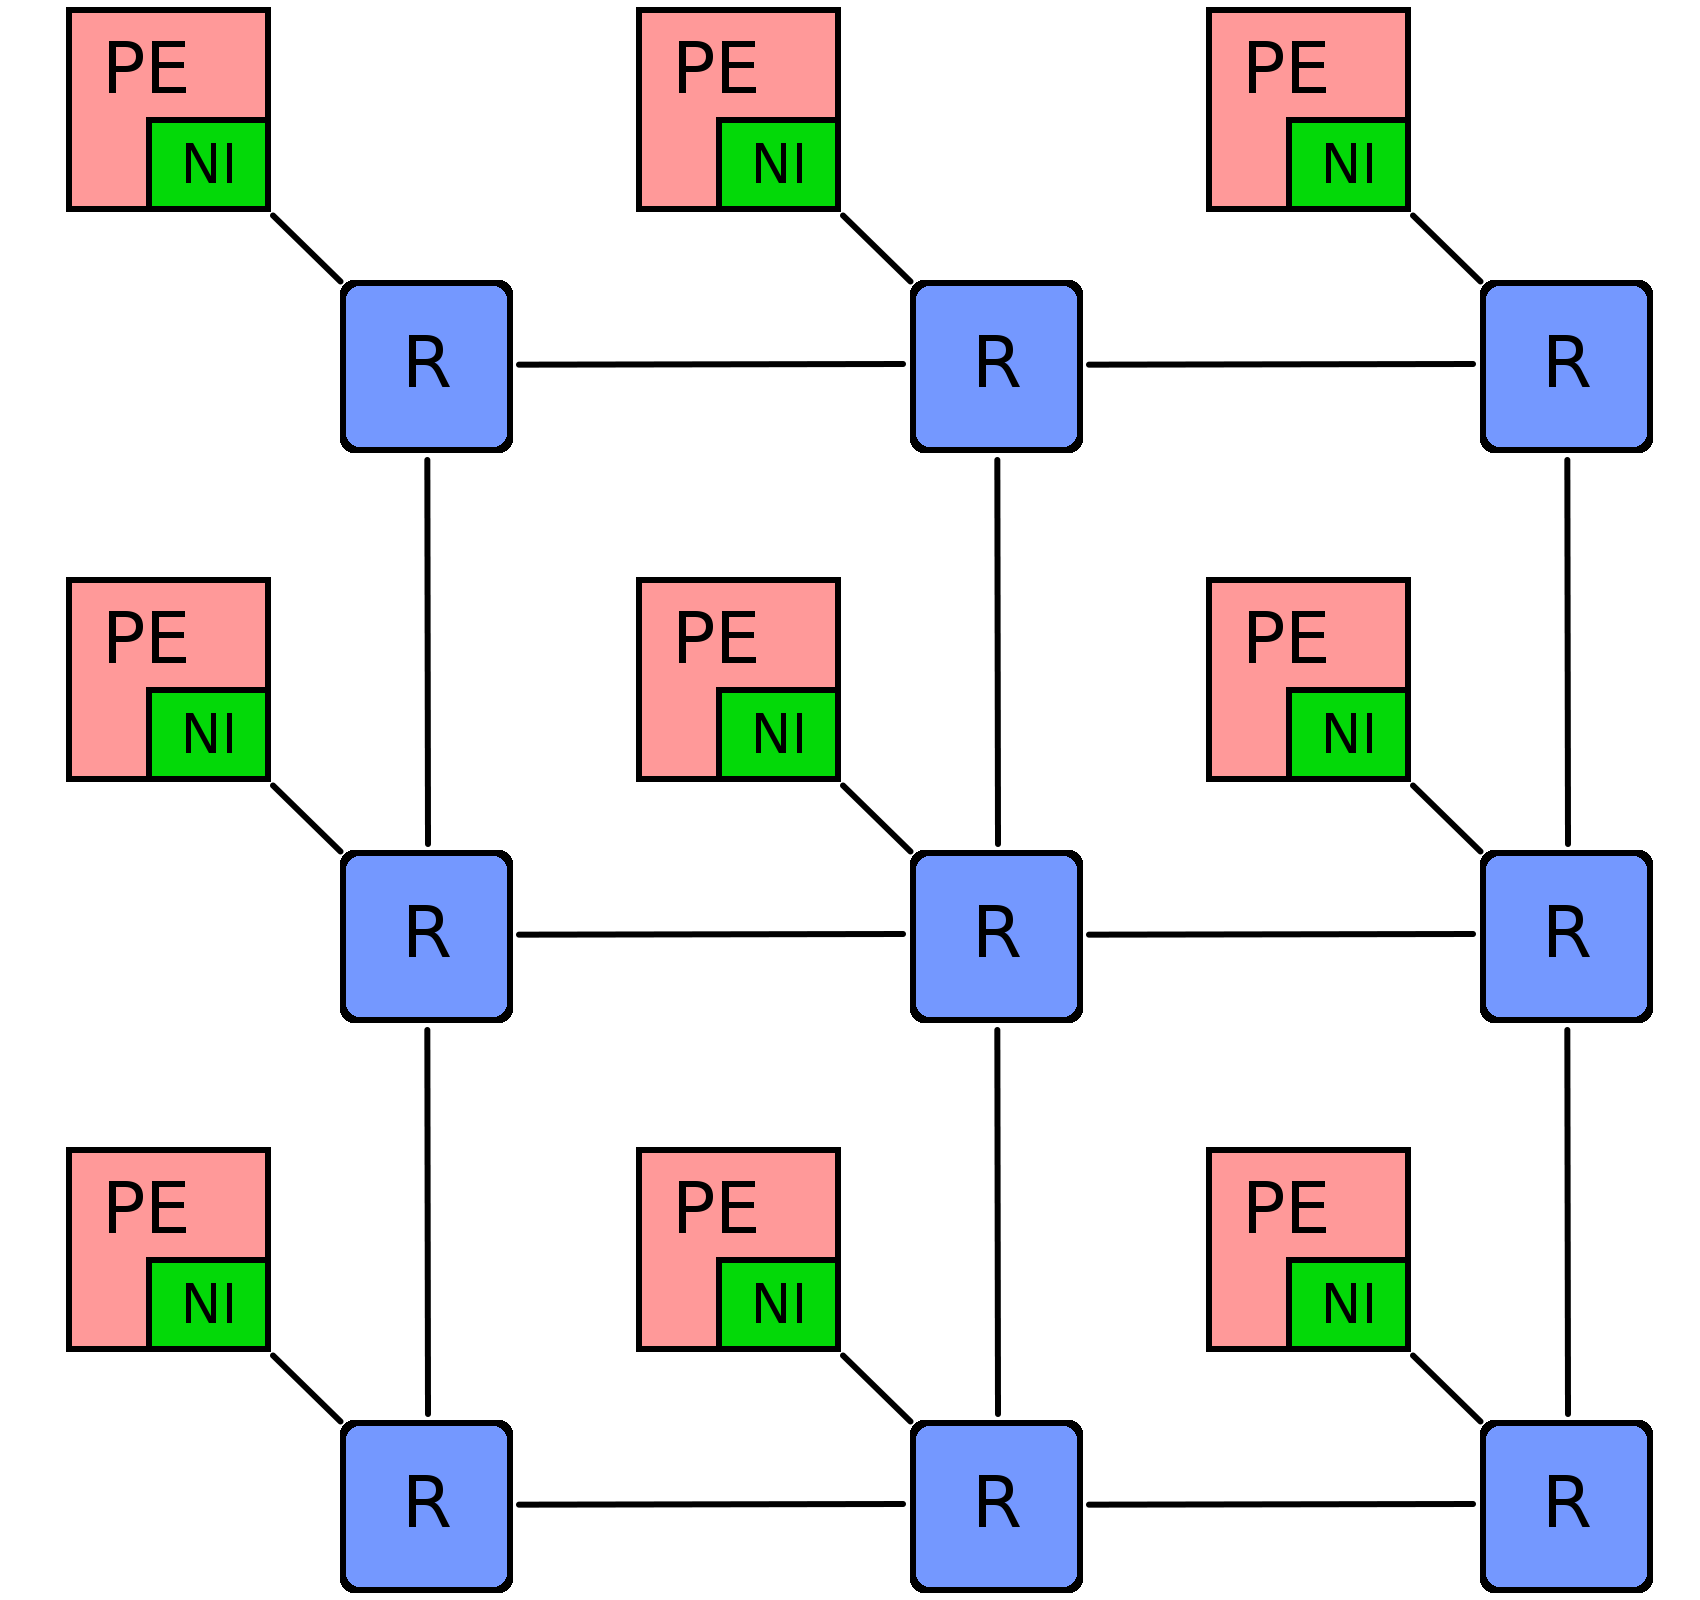
\includegraphics[width=0.6\textwidth]{noc_3x3_colored}
    \caption[Example of a 3x3 NoC]{Example of a 3x3 Network-on-Chip. The processing elements (red) contain a network interface
    (green), through which they are connected to a router (blue). The routers are connected in a 2D mesh topology.}
    \label{fig:nocexample}
\end{figure}

\section{Flits}\label{sec:flits}
Flits (short for \textit{flow control units}) are small pieces of data that are sent over a network. They are usually created by breaking a larger
packet down into parts that can be transmitted individually. \cite[6]{flitslecturecmu} Each flit must contain a set of headers (such as source and
destination address, sequence number, or identifier) that are required for routing and handling. \cite[2]{flitslectureutah} In addition, it contains
a payload that carries the actual information to be transmitted.

In the context of \glspl{noc}, flits are often used as the standard unit of transmission. \cite[51\psqq]{tatas16designingnocs} Details on how flits
are used in this thesis can be found in (insert section/chapter vref).
% TODO: insert reference

\section{Hardware Trojans}\label{sec:hardwaretrojans}
% What are HTs, why can they get into other hardware, what are their properties
Hardware trojans are \enquote{malicious modifications of electronic hardware} \cite[1]{bhunia14hardwaretrojans} with the intent of disrupting normal
system behavior or extract sensitive information. Because the integration of third party \gls{ip} has become increasingly popular due to circuit
complexity and cost efficiency \cites[1]{ancajas14fortnocs}[2]{bhunia14hardwaretrojans}, it is possible for adversaries to introduce hardware
trojans into larger systems, such as \glspl{mpsoc}.

In order to remain undetected, attackers aim to construct hardware trojans that are \enquote{stealthy in nature} \cite[1]{bhunia14hardwaretrojans}
and \enquote{evade […] detection through conventional postmanufacturing test} \cite[1]{bhunia14hardwaretrojans}. Hardware trojans are usually in a
dormant state until they are activated by a trigger signal to carry out their task. \cites{bhunia14hardwaretrojans}{ancajas14fortnocs} While the
trojan is inactive, communications through the \gls{noc} are unaffected and the system operates normally.

Attack types: information leak/eavesdropping, DoS (→ bandwidth depletion, deadlock, livelock)
% TODO: is this a fundamental? or write this when describing our attacker model?

\section{Network Coding}\label{sec:networkcodingfun}
Network coding is a technique for transmitting packets efficiently over a network. First described in 2003 by \citeauthor{li03linearnc}
\cite{li03linearnc}, the idea is to maximize the information flow through a network and achieve higher throughput than traditional transmission
schemes. It is achieved by allowing intermediate network nodes to encode incoming packets before passing them on, creating combinations of different
packets in the process. At the destinations, the received data can be decoded again to obtain the original packets.

A simple coding scheme, dubbed \textit{linear network coding}, is to regard all packets arriving at a node from different incoming links as a vector.
Then, linear transformations can be applied to it to obtain new combinations to send out. \cite[1]{li03linearnc} To allow receivers to decode the
combinations into the original packets, the encoding patterns applied at each node can be \enquote{agreed upon beforehand} \cite[1]{li03linearnc} or
can be attached to the packets in the form of a \textit{global encoding vector (\gls{gev})} \cite[5\psq]{chou07ncforinternetandwireless}.

In addition to increasing the network performance by maximizing throughput, network coding can also provide an additional layer of resilience against
malicious intermediate nodes. It facilitates \enquote{a natural way to take advantage of multipath diversity for security against wiretapping attacks}
\cite[8]{fragouli07ncfundamentals} and can also be helpful against active attackers.

During this thesis, network coding is used primarily as a means of resilience against attackers. Furthermore, only the sender nodes will compute
combinations of different flits, while intermediate nodes merely forward them. Section (insert vref here) illuminates this subject in detail.
